\documentclass[11pt,a4paper]{article}
\usepackage{amsmath}
\usepackage[utf8]{inputenc}
\usepackage[T1]{fontenc}
\usepackage{amsfonts}
\usepackage{amssymb}
\usepackage{graphicx} 
\usepackage{caption}
\usepackage{float}
\usepackage{url}
\author{Klara Muzalewska}

\title{Text prezentcji na sempowisko 2017 rok}


\begin{document}
\paragraph{}
Nazywam się Klara Muzalewska. Temat mojej prezentacji to:"Modelowanie budynku - chodź, pomóż mi AI"
\paragraph{}
Najpierw, powiem wam kilka zdań wprowadzających na temat modelowaniu budynku, następnie postaram się przedstawić jak można do tego procesu użyć sztucznej inteligencji na koniec przedstawie efekty uzyskane w tej pracy.
\paragraph{Modelowanie budynku}
Obecnie projektowanie budynków odbywa się przy pomocy technologii cyfrowego modelowania budynków - BIM (przez odpowiednie programy). Lecz wciąż jest to bardzo długi, iteracyjny proces wymagający dużej wiedzy inżynierow. Proces ten zależy również od wielu czynników zewnętrznych jak lokalizacja i tego jaka ma być funkcja danej modelowanej struktury.\\
W trakcie modelowania opieramy się na danych wcześniej modelowanych struktur. Jednym z źródeł takich danych jest Bridge Management Systems (BMS). Pytanie czy dzięki tak zebranym danym da się nabyć jakąś wiedze i czy może sie ona przydać do projektowania.\\
Oczywiście chidzi tou o nabywanie wiedzy przy pomocy AL.

\paragraph{Bayesian network}
Jest wiele metod do reprezentowania wiedzy w sieciach. Jedną z nich jest sieć Bayesowska. Jest ona oparta na teorii Byes'a, która przedstawia warunkowe prawdopodobieństwo P(A|B) wystąpienia zdarzenia A jeśli zdarzenie B.\\
\begin{center}
$P(A|B)=\frac{P(B|A)P(A)}{P(B)}$
\end{center}
Bayesowska sieć jest definiowana przez skierowany, acykliczny graf (DAG), gdzie każdy węzeł reprezentuje dyskretną lub ciągłą 
losową wartość \\
X=$\lbrace{X}_{1}, \ldots, {X}_{n}\rbrace$, a wierzchołki E reprezentują warunkową zależność pomiędzy wartościami.\\
Bezpośredni link z węzła X do Y mówi że X jest rodzicem Y. Strzałka pomiędzy dwoma wartościami jest zwykle interpretowana jako bezpośredni wpływ X na Y. Jeśli brak węzła, nie ma zależności. \\
Gdy mamy zdefiniowaną topologie grafu, każdy węzeł grafu jest powiązany z warunkowym prawdopodobieństwiem: $P = ({X}_{i}|parents({X}_{i}))$, który deterinuje wpływ rodzica węzła. Prawdopodobieństwa są oznaczone w tablicy prawdopodobieńst warunkowych (CPT). \\
Aby stworzyć sieć Bayesowską trzeba zrobić dwie rzeczy. Najpierw musimy nauczyć sieć struktury a następnie obliczyć A-priori warunkowe rozkłady prawdopodobieństwa dla każdego węzła.\\
Po stworzeniu możliwe jest wnioskowanie probalistyczne.\\
W naszym przypadku oznacza to że pobieramy zestawy danych z BMS, aby poznać strukturę sieci i obliczyć
tabele rozkładu prawdopodobieństwa, a następnie wykonujemy wnioskowani probabilistyczne dla nowego projektu mostu.

Możliwe jest zdefiniowanie struktury grafów sieci bayesowskiej poprzez uczenie się z zestawów treningowych w automatyczny sposób. Uzywa się do tego algorytmów takich jak algorytm wyszukiwania oparty na CI, algorytm K2 (Cooper i wsp. 1992), The Tree Augmented Naive Bayes (TAN). TAN tworzy strukturę sieci w następujący sposób:\\
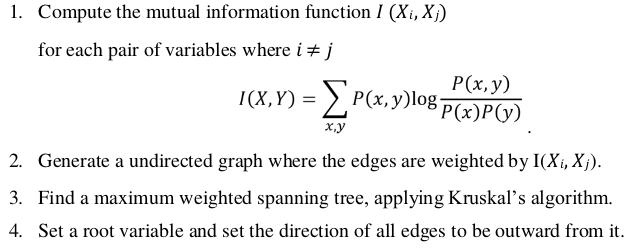
\includegraphics[scale=0.5]{TAN.png}\\
Do następnego kroku - przybliżonego wnioskowania- używamy próbkowania Gibbsa (który jest dobry do Beyesowskich sieci).
Próbkowanie Gibbsa:\\
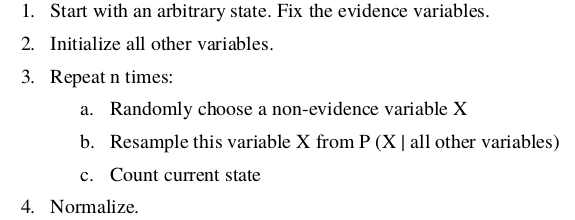
\includegraphics[scale=0.5]{Gibs.png} 

\paragraph{Nasze wyniki}
Niestety do tej pory nie można było użyć danych z BMS wiec do tworzenia sieci wykorzystany został zestaw randomowych danych   przy pomocy bazy znanych danych. \\
Aby dostać sensowne dane wygenerowane zostały 10000 zestawów danych treningowych. \\
Wyniki były odpowiednie do zamodelowania pewnych mostów. Aby uzyskać lepsze rady dotyczące projektowania należałoby dodać więcej danych i lepsza dyskretyzacja. Aby  uwzględnić kolejne procesy projektowania należałoby uwzględnić kolejne czynniki, które możemy uzyskać również z BMS. Dzięki temu możemy lepiej odpowiedzieć na pytanie jaki typ konstrukcji dobrze działa w danych warunkach i przy danym koszcie.
\paragraph{Bibliografia}
Aby przygotować prezentacje, korzystałam z artykułu: "Knowledge based Bridge Engineering - Artificial Intelligence meets Building Information Modeling" Dominic Singer, Maximilian Bügler, André Borrmann. 

\end{document}